\documentclass[12pt]{article}
% load the necessary packages
\usepackage[spanish]{babel}
\usepackage[latin1]{inputenc}
\usepackage[paperheight=26.67cm,paperwidth=36.15cm,margin={0pt,0pt},bindingoffset=-6mm]{geometry}
\usepackage[dvipsnames,prologue,table]{pstricks}
\usepackage{pst-all}
\usepackage{pst-grad}
\usepackage{graphicx}
\usepackage{rotating}
\usepackage{color}
\usepackage{calc}
%\usepackage[ISBN=978-80-85955-35-4]{ean13isbn}
%\EANisbn[SC4]

\usepackage{fp}

\makeatletter

\FPset{margenancho}{0.32}
\FPset{margenalto}{0.335}
\FPset{alto}{26}
\FPset{ancho}{16.82}
\FPset{lomo}{1.867}
\FPset{iniciolomo}{17.14}
\FPset{anchobandamaroonportada}{2.3}
\FPset{anchobandawhitecontraportada}{2.7}
\FPset{anchobanda}{2}
\FPset{widthUGR}{5.446} %5.046
\FPset{widthETSIIT}{1.45}
\FPset{widthoATC}{5.477}
\FPset{altoescudos}{1}
\FPset{cuadrofotobiografia}{7.8}

\FPeval{altocompleto}{\margenalto + \alto + \margenalto}
\FPeval{anchocompleto}{\margenancho + \ancho + \lomo + \ancho + \margenancho}
\FPeval{inicioportada}{\margenancho + \ancho + \lomo}
\FPeval{contraportada}{\margenancho}
\FPeval{bandamaroonportada}{\inicioportada + \anchobandamaroonportada}
\FPeval{altomenosmargen}{\altocompleto - \margenalto}
\FPeval{anchomenosmargen}{\anchocompleto - \margenancho}

\FPeval{centrolomo}{(\iniciolomo + \inicioportada)/ 2}
\FPeval{centrolomosuperior}{\centrolomo + 0.3}
\FPeval{centrolomoinferior}{\centrolomo -0.3}

\FPeval{financhobandacontraportada}{\anchobandawhitecontraportada + \anchobanda}
\FPeval{letraswhitebandacontraportada}{\financhobandacontraportada - 0.2}
\FPeval{letrasmaroonbandacontraportada}{\financhobandacontraportada -1.15}

\FPeval{financhobandaportada}{\bandamaroonportada}
\FPeval{letraswhitebandaportada}{\financhobandaportada - 1.0}
\FPeval{letrasmaroonbandaportada}{\financhobandaportada -0.1}

\FPeval{mitadblancaportada}{(\anchocompleto + \financhobandaportada) / 2 }
\FPeval{mitadportadadesplazada}{\mitadblancaportada + 1}

\FPeval{mitadmarooncontraportada}{(\financhobandacontraportada + \iniciolomo) / 2 }
\FPeval{mitadcontraportadadesplazada}{\mitadmarooncontraportada + 1}

\FPeval{fotobiografia}{\cuadrofotobiografia + 0.1}
\FPeval{fincuadrofotobiografia}{\cuadrofotobiografia + 1.2}
\FPeval{textobiografia}{\fincuadrofotobiografia + 0.2}

\FPeval{anchoUGR}{\iniciolomo - 0.2}
\FPeval{anchoETSIIT}{\anchoUGR - \widthUGR - 0.2}
\FPeval{anchoATC}{\anchoETSIIT - \widthETSIIT}

% begin the document and suppress page numbers
\begin{document}
%\pagecolor{Maroon}
\pagestyle{empty}
% create the box with the front cover picture
\newsavebox\IBox
\sbox\IBox{
\includegraphics[width=14cm]{gfx/bordesLogoUGRcover.eps}}

\newsavebox\UGRBox
\sbox\UGRBox{
\includegraphics[height=1.7cm]{gfx/logougr.eps}}

\newsavebox\ETSIITBox
\sbox\ETSIITBox{
\includegraphics[height=1.7cm]{gfx/logoetsiit.eps}}

\newsavebox\ATCBox
\sbox\ATCBox{
\includegraphics[height=1.7cm]{gfx/logoatc.eps}}


% set up the picture environment
\psset{unit=1cm}

\begin{pspicture}(0,0)(\anchocompleto,\altocompleto)
\psframe[fillstyle=solid,fillcolor=Maroon,linewidth=0pt,linecolor=Maroon](0,0)(\bandamaroonportada,\altocompleto)

\newfont{\TituloPrincipalFont}{pncb scaled 4500}%{eurb10 scaled 7000}%
\newfont{\TituloSegundoFont}{pncb scaled 7805}%{pncb scaled 4500}%{eurb10 scaled 7000}%

% place the front cover picture
\rput[c]{45}(33cm,3cm){\usebox\IBox}

% Letras montadas sobre banda Maroon
\rput[lt]{90}(\letraswhitebandaportada,3.7){\TituloPrincipalFont \color{white}{Universidad de Granada}}
\rput[lt]{90}(\letrasmaroonbandaportada,3.7){\TituloSegundoFont \color{Maroon}{Tesis Doctoral}}

% put the text on the front cover
\newsavebox\Titlebox
\sbox\Titlebox{\begin{minipage}{11cm}
\centering\textcolor{black}{\textsc{\Large Extracci\'on Eficiente de la\\ Estructura de Escenas Naturales}}
\end{minipage}}

\rput[ct](\mitadportadadesplazada,20){\usebox\Titlebox}
\rput[ct](\mitadportadadesplazada,19){\color{black}{\textsc{\normalsize Jos\'e Manuel Palomares Mu\~noz}}}
\rput[c](\mitadblancaportada,25.5){\textsc{\footnotesize Departamento de Arquitectura y Tecnolog\'{\i}a de Computadores}}
\rput[c](\mitadblancaportada,25.2){\textsc{\scriptsize Escuela T�cnica Superior de Ingenier�as Inform�tica y de Telecomunicaci�n}}
\rput[c](\mitadblancaportada,24.9){\textsc{\scriptsize Universidad de Granada}}


% put the text on the spine (note the rotation over 270 degrees)

\rput[c](\centrolomo,23){ \begin{turn}{-90}
{
\color{white} {\Large Tesis Doctoral}
} \end{turn} }

\rput[c](\centrolomosuperior,14){ \begin{turn}{-90}
{
\color{white} \textsc{\small Extracci�n Eficiente de la Estructura de Escenas Naturales}
} \end{turn} }

\rput[c](\centrolomoinferior,14){ \begin{turn}{-90}
{
\color{white} \textsc{\footnotesize Jos\'e Manuel Palomares Mu\~noz}
} \end{turn} }

\rput[c](\centrolomo,2.5){\color{white}\textbf{2011}}

% Then we close all open environments
% 
% %%%%%%%%%%%%%%%%%%%%%%%%%%%%%%%%%%

\psframe[fillstyle=solid,fillcolor=white,linewidth=0pt,linecolor=white](\anchobandawhitecontraportada,0)(\financhobandacontraportada,\altocompleto)
\rput[rb]{270}(\letraswhitebandacontraportada,3.7){\TituloSegundoFont \color{white}{Tesis Doctoral}}
\rput[rb]{270}(\letrasmaroonbandacontraportada,3.7){\TituloPrincipalFont \color{Maroon}{Universidad de Granada}}

\rput[rb](\anchoUGR,\altoescudos){\usebox\UGRBox}
\rput[rb](\anchoETSIIT,\altoescudos){\usebox\ETSIITBox}
\rput[rb](\anchoATC,\altoescudos){\usebox\ATCBox}

\newsavebox\Authorbox
\sbox\Authorbox{\includegraphics[width=2cm]{gfx/jmpalomares.eps}}

% A white box in which place the photo
\psframe[fillstyle=solid,fillcolor=white](\cuadrofotobiografia,21.6)(\fincuadrofotobiografia,23.4)
% now place the picture
\rput[lt](\fotobiografia,23.3){\usebox\Authorbox}
% create a savebx for the biography. The width has been adjusted so
% that the right margin matches with that of the book blurb
\newsavebox\Biobox
\sbox\Biobox{\begin{minipage}{6.5cm}
\textcolor{white}{\scriptsize \textsc{Jos\'e Manuel Palomares Mu\~noz} es Diplomado y Licenciado en Inform�tica por la Universidad de Granada en 1996 y 1998 respectivamente. Desde el 2000 trabaja en el \'Area de Arquitectura y Tecnolog�a de Computadores de la Universidad de C�rdoba donde imparte docencia de ``Inform�tica Industrial'', ``Arquitectura de Computadores'' y ``Sistemas en Tiempo Real''. Su e-mail de contacto es: \texttt{jmpalomares@uco.es}}
\end{minipage}}
% and put it where it belongs
\rput[tl](\textobiografia,23.5){\usebox\Biobox}

% Create a Box containing the text for the back cover
\newsavebox\Blurbbox
\sbox\Blurbbox{\begin{minipage}{8.5cm}
\textcolor{white}{{\huge E}\footnotesize\textsc{sta} Tesis Doctoral pretende proporcionar un mecanismo que permita la extracci�n eficiente de las caracter�sticas presentes en una escena natural para pacientes con \textsc{Baja Visi�n}. Este trabajo presenta la adaptaci�n del operador \emph{convoluci�n} bajo el paradigma \textsc{LIP}, de tal forma que permite la construcci�n de m�todos basados en filtros separables en dicho paradigma. Debido al car�cter logar�tmico de \textsc{LIP}, gracias a este operador se pueden dise�ar algoritmos de extracci�n de contornos invariantes ante cambios de iluminaci�n. En este trabajo se adaptan diversos algoritmos de extracci�n de bordes tradicionales al paradigma \textsc{LIP} utilizando el operador propuesto.\\[1em]
\noindent {\huge U}\footnotesize\textsc{na} segunda gran aportaci�n es la evaluaci�n \textsc{Subjetiva} mediante cuestionarios de la calidad de los mapas de contornos obtenidos por cada m�todo. Se proponen una serie de recomendaciones para la construcci�n de buenas encuestas para la evaluaci�n de im�genes de contornos, que han sido utilizadas para evaluar la calidad de los m�todos adaptados al paradigma \textsc{LIP} utilizando el nuevo operador propuesto. La muestra poblacional que responde a dicha encuesta incluye tanto a individuos con un grado de \textsc{Visi�n Est�ndar} como a pacientes con \textsc{Baja Visi�n}.}
\end{minipage}}
% And position the box
\rput[c](\mitadcontraportadadesplazada,12){\usebox\Blurbbox}

% %L�nea discont�nua de borde
% \psframe[linewidth=1pt,linestyle=dotted,linecolor=black,fillstyle=none](\margenancho,\margenalto)(\anchomenosmargen,\altomenosmargen)
% 
% %Marcas de doblez de la contraportada
% \psline(\margenancho,0)(\margenancho,\margenalto)
% \psline(0,\margenalto)(\margenancho,\margenalto)
% \psline(\margenancho,\altocompleto)(\margenancho,\altomenosmargen)
% \psline(0,\altomenosmargen)(\margenancho,\altomenosmargen)
% 
% %Marcas de doblez de la portada
% \psline(\anchomenosmargen,0)(\anchomenosmargen,\margenalto)
% \psline(\anchomenosmargen,\margenalto)(\anchocompleto,\margenalto)
% \psline(\anchomenosmargen,\altocompleto)(\anchomenosmargen,\altomenosmargen)
% \psline(\anchocompleto,\altomenosmargen)(\anchomenosmargen,\altomenosmargen)
% 
% %Marcas de doblez del LOMO
% \psline(\iniciolomo,0)(\iniciolomo,\margenalto)
% \psline(\inicioportada,0)(\inicioportada,\margenalto)
% \psline(\iniciolomo,\altocompleto)(\iniciolomo,\altomenosmargen)
% \psline(\inicioportada,\altocompleto)(\inicioportada,\altomenosmargen)


\end{pspicture}

\end{document}
